\documentclass{pracamgr}

\usepackage{amsmath, amsfonts,amssymb,amsthm,epsfig,epstopdf,url,array,bm,color}

\usepackage{polski}
\usepackage[english,polish]{babel}
\usepackage[utf8]{inputenc}

\usepackage{verbatim}
\usepackage{lmodern}
\usepackage[section]{placeins}
\usepackage[font=small]{caption}

\usepackage{program}

%\usepackage{tikz}
%\usetikzlibrary{arrows}

% Dane magistranta:

\author{Marek Rogala}

\nralbumu{277570}

\title{Deklaratywne zapytania na dużych grafach i ich rozproszone wyliczanie}

\tytulang{Declarative queries on large graphs and their distributed evaluation}

\kierunek{Informatyka}

\opiekun{dra Jacka Sroki\\
  Instytut Informatyki\\
  }

\date{Wrzesień 2014}

\dziedzina{ 
11.3 Informatyka\\
}

\klasyfikacja{Information Systems: Query languages }

% Słowa kluczowe:
\keywords{Przetwarzanie dużych grafów, deklaratywne języki zapytań, obliczenia na dużych zbiorach danych, Datalog, SociaLite, Apache Spark, Hadoop. \\
Large graphs processing, Declarative query languages, Computations on large datasets, Datalog, SociaLite, Apache Spark, Hadoop}

\theoremstyle{plain}
\newtheorem{thm}{Theorem}[section]
\newtheorem{lem}[thm]{Lemma}
\newtheorem{prop}[thm]{Proposition}
\newtheorem*{cor}{Corollary}

\theoremstyle{definition}
\newtheorem{defn}{Definition}[section]
\newtheorem{conj}{Conjecture}[section]
\newtheorem{exmp}{Example}[section]

\theoremstyle{remark}
\newtheorem*{rem}{Remark}
\newtheorem*{note}{Note}

\newcommand{\todo}[1]{\textcolor{red}{@TODO: #1}}

\newcommand{\datalogra}{Datalog$^{RA}$ }
\newcommand{\datalogneg}{Datalog$^{\neg}$ }
\newcommand{\aggfun}{\textit{aggfun} }
\newcommand{\aggcol}{\textit{aggcol} }
\newcommand{\assign}{:-}

\def\changemargin#1#2{\list{}{\rightmargin#2\leftmargin#1}\item[]}
\let\endchangemargin=\endlist 

\newenvironment{centab}[1]{\begin{center}\begin{tabular}{#1}}{\end{tabular}\end{center}}


\newcommand{\narrow}[1]{\begin{changemargin}{2cm}{2cm} #1 \end{changemargin}}
\newcommand{\relat}[2]{$\textsc{#1}#2$}
\newcommand{\rdprog}[2]{
  \narrow{
      #1
      \begin{flalign*}
      #2
      \end{flalign*}
    }
}
\newcommand{\dprog}[4]{
  \begin{figure}[h!]
    \narrow{
      #1
      \begin{flalign*}
      #2
      \end{flalign*}
      \caption{#3}
      \label{#4}
    }
\end{figure}

}

% koniec definicji

\begin{document}
\maketitle

\begin{abstract}
W pracy przedstawiono metodę tłumaczenia programów zapisanych w Datalogu
i jego rozszerzonych wersjach do programów w modelu obliczeniowym Google Pregel,
oraz implementację prototypowego kompilatora wykorzystującego tę metodę do uruchamiania takich programów na platformie Apache Spark.
Takie podejście pozwala na wykonywanie obliczeń na istniejących architekturach do obliczeń rozproszonych
za pomocą deklaratywnego języka zapytań, znacznie prostszego niż dotychczas dostępne języki dla tych architektur.
\end{abstract}

\tableofcontents
%\listoffigures
%\listoftables

\chapter*{Introduction}
\addcontentsline{toc}{chapter}{Introduction}
In recent years, the humanity has created many graph datasets much larger than those available ever before.
Those graphs became a very popular object of research. Most notable examples are \emph{the Web graph} -- a graph of Internet websites and links between them as well as all kinds of social networks. Other interesting graphs include transportation routes, similarity of newspaper of scientific articles or citations among them.

With increasing computational power and memory space, we can expect more and more real-life graphs to became subject to computation. We can also expect the existing graphs, such as the Web or social networks, to grow in all aspects.

The graphs mentioned can be a source of a huge amount of useful information. Hence, there is an increasing number of practical computational problems.
Some of the analyses carried out are ranking of the graph nodes, e.g. importance of a Web page, determining most influential users in given group of people, detecting communities with clustering, computing metrics for the whole graph or some parts of it and connection predictions.
Usually, such analyses are built on top of standard graph algorithms, such as variations of PageRank \cite{pagerank}, shortest paths or connected components.

When dealing with so large graphs, distribution of the computations among many machines is inevitable. The graph size is often be too large to fit in one computer's memory. At the same time, performing useful computations on a single machine would take too much time for it to be a feasible solution. Sizes of the graphs are growing faster than the computational power of a computer, and so is the need for distributing the computations.

In the past, we have seen many tools for efficient distributed large dataset computations, such as Google's MapReduce \cite{mapreduce} and its widely used open source counterpart, Apache's Hadoop, as well as higher-level languages such as PigLatin and Hive. However, those are not well suited for graph computations, as they do not support iteration well.

Recently, there is an outbreak of frameworks and languages for large graphs processing, including industrial systems such as Google's Pregel \cite{pregel}, its open-source version Apache Giraph and Spark GraphX, Giraph++ \cite{giraphpp}.

The frameworks currently available allow one to implement a graph algorithm in a specified model, for example Pregel's "think like a vertex", using a programming language like Java, Scala or Python. On the other hand, query languages, such as SQL, are a bad fit for graph data because of limited support of iteration. One of the advantages of query languages over general-purpose programming languages is that they are available for a much broader group of users: they are used not only by programmers, but also by analysts and data scientists. Queries are often optimized by the query engines automatically. With the rise of graph computational problems, we need an easier way to extract information from graphs: a query language for effectively expressing data queries typical for graphs.

The Socialite \cite{socialite, distsoc} language is one of the most interesting propositions. It is based on a classical language --- Datalog \cite{fod}. In Datalog, the problem is expressed in a declarative way as a set of rules. Declarative semantics makes it easy to distribute the computations, since no execution flow is embedded in the program code. It also gives many possibilities for optimizations and approximate evaluation. At the same time, Datalog's support for recursion is crucial, since most graph algorithms have iterative nature. However, most practical graph algorithms can not be expressed efficiently in Datalog because of the language limitations. With a few extensions to original Datalog, most important of which is recursive aggregation, SociaLite makes it easy to write intuitive programs which can be executed very efficiently.

Unfortunately, there is no solid implementation of SociaLite available. The interpreter published by the authors is undocumented and contains many bugs. It is hard to imagine it being implemented in the industry in the foreseeable future. At the same time, papers \cite{socialite} and \cite{distsoc} which introduced SociaLite contain certain simplifications and are not specific about some important details in definitions and proofs.

The goal of this work is to bridge the gap between the theoretical idea for SociaLite and a practical implementation and to draw a path towards its usage in the industry. We show how to translate SociaLite declarative programs into Pregel "think-like-a-vertex" programs and introduce a compiler that enables SociaLite programs to be executed on existing infrastructure. This allows its users to write and execute SociaLite programs without any additional effort to build a dedicated server infrastructure for that.

This works presents an experimental implementation of the SociaLite language on the Apache Spark platform. Spark is an open-source project which provides a general platform for processing large datasets which has gained a huge momentum since the initial white paper in 2010 \cite{spark} and inclusion into Apache Incubator in June 2013. Distinctive features of Spark are the ability keep cached data in nodes memory, which gives impressive speedups over other environments like Hadoop MapReduce and a powerful API allowing for various usages including MapReduce, machine learning, computations on graphs and stream data processing. In February 2014 Spark became a top-level project of the Apache Foundation, and in since July 2014 it is included in the Cloudera CDH, a popular enterprise platform for Hadoop deployment. Spark is already a stable, well-tested platform which is being intensively developed and can be expected to become a new industry standard in large datasets processing. For these reasons, it has been chosen as the most promising implementation platform for the S2P compiler.

The work consists of six chapters. In Chapter~\ref{r:datalog} we recall definitions of Datalog and its evaluation methods while Chapter~\ref{r:pregel} contains an introduction to the Pregel computation model. In Chapter~\ref{r:socialite} we describe the extensions introduced by SociaLite and provide formal definitions and general-case proofs which the original papers lack. Chapter \ref{r:s2p} shows the translation procedure from SociaLite to Pregel programs implemented in the S2P compiler, which is described in Chapter~\ref{r:implementation}. In Chapter~\ref{r:summary} we sketch the possible future work and the path to industrial implementation of the language using the S2P compiler.

\section{Basic definitions}\label{r:basicdefs}
Let us give some basic definitions which will be used in this paper.

The languages considered in the paper operate on databases, which consist of relations identified by relation names. The databases can contain any value from an countable infinite set $\textbf{dom}$ called the \emph{domain}. The programs use variables from a set $\bf{var}$, which is disjoint from $\bf{dom}$.

\begin{defn}
A \emph{database schema} is a collection of relation names $R$ with arity $ar(R) \ge 0$ defined for each relation.

Given a database schema $\sigma$, let $R$ is a relation in $\sigma$ with arity $n$. A \emph{fact} over $R$ is an expression $R(x_1 , \dots , x_n)$, where each $x_i \in \textbf{dom}$. A fact is sometimes written in the form $R(v)$ where $v \in \textbf{dom}^n$ is a tuple. A \emph{relation} or \emph{relation instance} over $R$ is defined as a finite set of facts over $R$.

A \emph{database instance} $I$ over database schema $\sigma$ is a union of relations over $R$, where $R \in \sigma$.

Elements of $\bm{dom}$ are called \emph{constants}, whereas elements of $\bf{var}$ are called \emph{(free) variables}.
\end{defn}

\begin{defn}
If $f$ is a function $f: D \to D$ and $f(x) = x$ for an $x \in D$, then $x$ is called a \emph{fix-point} of $f$.
\end{defn}

\todo{valuation}


\chapter{Datalog}\label{r:datalog}

In this chapter we describe the basic Datalog language and its typical extended versions.

Languages based on relational algebra and relational calculus, like SQL, are widely used and researched as query languages for relational databases. This dates back to Edgar F. Codd's relational model \cite{coddrelmodel} introduced in 1970. Unfortunately, such languages leave some simple operations that they can not handle. Examples of such problems are transitive closure of a graph or distances from a vertex to all other vertices.

Datalog is a language that enhances relational calculus with recursion, which allows for solving those problems. It appeared around 1978 and is inspired by logical programming paradigm. Recently, there is an increasing interest in Datalog research as well as its implementations in industry. Datalog is typically extended with negation and simple, non-recursive aggregation.

Let us begin with an example of a problem which can not be solved in relational calculus, but can be easily solved in Datalog.

Let us suppose that we have a database with a binary relation $\textsc{Edge}$. The database represents a graph $G$: if $\textsc{Edge}(a, b)$ means that there is an edge in $G$ between vertices $a$ and $b$. Given a selected vertex $s$, we would like to find all vertices in $G$ that are reachable from $s$.

Unfortunately, unless we have some additional assumptions about $G$, is seems difficult to answer this query using languages like SQL. It can be proven that this kind of query is not expressible in the relational calculus \cite{fod}. Intuitively, what is necessary to answer such queries is some kind of conditional iteration or recursion, which is the most important feature of Datalog.

\section{History}

Datalog is not credited to any particular researchers since it originated as an extension or restriction of various other languages, including logic programming languages. It emerged as a separate area of research around 1977. It is believed that professor David Maier is the author of the name \emph{Datalog}.

Datalog is described in detail in classical books on databases theory, such as \emph{Foundations of Databases} \cite{fod}.

The language has been proven to be useful in various fields like program analysis \cite{pointanalysis}, network systems \cite{boomanalysis, dataloganalysis}. It is also used to formally define computational problems which can be solved with different models and frameworks, allowing for comparison of those frameworks and their optimizations \cite{ullman}. 

Some of the most important fields of research concerning Datalog are optimizations in programs evaluation (magic sets \cite{magicsets}, subsumptive queries \cite{subsumptivequeries}) and extensions to the language \cite{magicsetsexist, disjunctivedatalog, datalogrelaunched}.

Recently there is also an increasing interest in applications of Datalog in industry. Two examples worth mentioning are LogicBlox and Datomic. LogicBlox \cite{logicblox} delivers a high performance database which can be queried with a Datalog variant called LogiQL.  Datomic \cite{datomic} is a distributed database with an innovative architecture featuring immutable records and temporal queries, which uses Datalog as a query language.

\section{Introduction to Datalog}

Before we formally define Datalog syntax and semantics, let us take a look at an example program in this language.

As before, let us assume that the database contains a relation $\textsc{Edge}$ representing a graph and $\textsc{Edge}(a, b)$ means that there is an edge between vertices $a$ and $b$. The following program computes relation $\textsc{Tc}$ containing a transitive closure of relation $\textsc{Edge}$.

\dprog{}{
  & \textsc{Tc} (a, b) &&  & \assign & && \textsc{Edge} (a, b). & \\
  & \textsc{Tc} (a, b) &&  & \assign & && \textsc{Tc} (a, c), \textsc{Edge}(c, b). &\\
}{Datalog query for computing transitive closure of a graph}{ex:tcdatalog}

This program contains two rules. The first one states that if there is an edge between $a$ and $b$, then also there is such edge in the transitive closure. The second rule says that if there is a connection in the transitive closure between $a$ and some $c$ and at the same time there is an edge between $c$ and $b$ in the original graph, then there also exists a connection in transitive closure between $a$ and $b$. This is where recursion is used: $\textsc{Tc}$ appears on both sides of the second rule.

For example, let $\textsc{Edge}$ contain the following tuples:

\begin{centab}{ | c | }
  \hline
  $\textsc{Edge}$ \\
  \hline
  $(1, 2)$ \\
  $(2, 3)$ \\
  $(3, 4)$ \\
  $(2, 5)$ \\
  \hline
\end{centab}

The result of the program is:

\begin{centab}{ | c | }
  \hline
  $\textsc{Tc}$ \\
  \hline
  $(1, 2)$ \\
  $(1, 3)$ \\
  $(1, 4)$ \\
  $(1, 5)$ \\
  $(2, 3)$ \\
  $(2, 4)$ \\
  $(2, 5)$ \\
  $(3, 4)$ \\
  \hline
\end{centab}

As we can see, the program defines a function from the an instance of relation $\textsc{Edge}$ into an instance of relation $\textsc{Tc}$.

In the following sections, we will define Datalog's syntax and semantics in a more formal way.

\section{Datalog syntax}
Let us formally Datalog programs and rules.

\begin{defn}
A \emph{rule} is an expression of the form:
$$ \textsc{R}(x) \assign R_1(x_1), \dots, R_n(x_n). $$
where $n \ge 1$, $R, R_1, \dots, R_n$ are names of relations and $x, x_1, \dots x_n$ are tuples of free variables or constants. Each tuple $x, x_1, \dots x_n$ must have the same arity as the corresponding relation.
\end{defn}\label{d:datalogrule}

The sign $\assign$ splits the rule into two parts: the leftmost part, i.e. $R(x)$ is called the \emph{head} of the rule, while the rightmost part, i.e. $R_1(x_1), \dots, R_n(x_n)$ is called the \emph{body} of the rule. The elements of body separated by commas are called \emph{subgoals}. Head and the subgoals are called \emph{atoms}. Each atom consists of a \emph{predicate}, i.e. the relation name and \emph{arguments}.

\begin{defn}
A rule is \emph{safe} if the each free variable appearing in its head also appears in at least one of the subgoals.
\end{defn}\label{d:datalogsaferule}

\begin{defn}
A \emph{program} in Datalog is a finite set of safe rules.
\end{defn}\label{d:datalogprog}

By $adom(P)$ we denote the set of constants appearing in the rules of $P$.

The \emph{schema} of program $P$ is the set of all relation names occurring in $P$ and is denoted by $sch(P)$.

\begin{defn}
The rules of a Datalog program $P$ divide the relations into two disjoint classes: 
\begin{itemize}
\item \emph{extensional} relations, i.e. relations that occur only in the subgoals, but never in the head of the rules in $P$
\item \emph{intensional} relations occurring in the head of at least one of the rules in $P$
\end{itemize}
\end{defn}

The set of extensional relations are called the \emph{edb} or \emph{extensional database}, whereas the set of intensional relations is called \emph{idb} or \emph{intensional database}. For a program $P$, the \emph{extensional database schema}, denoted by $edb(P)$, is the set of all extensional relation names. Similarly, the \emph{intensional database schema}, denoted by $idb(P)$, is the set of all intensional relation names. 

A Datalog program is essentially a function from database instances over $edb(P)$ into database instances over $idb(P)$.

\begin{defn}
Given a rule $ \textsc{R}(x) \assign R_1(x_1), \dots, R_n(x_n). $, if $\nu$ is a valuation of variables appearing in this rule, then we obtain an \emph{instantiation} of this rule by replacing each variable $t$ in the rule by its value $\nu(t)$:
$$ \textsc{R}(\nu(x)) \assign R_1(\nu(x_1)), \dots, R_n(\nu(x_n)). $$
\end{defn}

\begin{exmp}
As an example, let us consider the following program $P$:

\rdprog{}{
  & \textsc{Mother} (parent, child) &&  & \assign & && \textsc{Parent}(parent, child), \textsc{Woman}(parent) & \\
  & \textsc{Father} (parent, child) &&  & \assign & && \textsc{Parent}(parent, child), \textsc{Man}(parent) & \\
  & \textsc{Ancestor} (ancestor, child) &&  & \assign & && \textsc{Parent} (ancestor, child) &\\
  & \textsc{Ancestor} (ancestor, child) &&  & \assign & && \textsc{Ancestor} (ancestor, parent), \textsc{Parent} (parent, child) &\\
}{}{}

Assuming that \relat{Parent}{(p, c)} means that $p$ is $c$'s parent and \relat{Woman}{(x)} and \relat{Man}{(x)} tell whether person $x$ is a woman or a man, this program computes child's father, mother and all its ancestors that can be derived.

\emph{edb} and \emph{idb} for $P$ are the following:
\begin{align*}
edb(P) =& \{\textsc{Parent}, \textsc{Man}, \textsc{Woman}\} \\
idb(P) =& \{\textsc{Mother}, \textsc{Father}, \textsc{Ancestor}\}
\end{align*}

\relat{Parent}{}, \relat{Man}{}, \relat{Man}{} are \emph{edb} relations, because there are no rules for those relations. All of their contents must be provided as an input. On the other hand, \relat{Mother}{}, \relat{Father}{}, \relat{Ancestor}{} are \emph{idb} relations, since there are rules for computing them. Only one of them, \relat{Ancestor}{} is recursively defined.

If $Anna, Chris, Patrick$ are some values in the domain, an example of an instantiation of the last rule is:
$$\textsc{Ancestor}(Anna, Chris) \assign \textsc{Ancestor} (Anna, Patrick), \textsc{Parent} (Patrick, Chris)$$
\end{exmp}

\subsection{Differences between Datalog and Prolog}
Despite the close relation between Datalog and logic programming languages, there are some significant differences:
\begin{itemize}
\item in Prolog, one can use complex terms as arguments to predicates, for example $p(s(x), y)$, which is not permitted in Datalog, where the only allowed arguments are domain elements or variables: $p(x, y)$.
\item in Prolog, there is a cut operator which is not present in Datalog. While some versions of Datalog have the notion of negation, but it is still different than the cut operator.
\item Datalog requires the rules to be \emph{safe}, which means that every variable mentioned in a rule must be also mentioned at least once in a non-negated, non-arithmetic sense
\item 
\end{itemize}


\section{Datalog semantics}
Semantics of a Datalog program can be defined using one of three different equivalent approaches.

In the \emph{model theoretic} definition, we consider the rules of program $P$ to be logical properties of the desired solution. From all possible instances of the intensional database we choose those, which are a \emph{model} for the program, i.e. satisfy all the rules. The smallest such model is defined to be the semantics of $P$.

A second approach is \emph{proof theoretic}, in which a fact is included in the result if and only if it can be derived, or proven using the rules. There are two strategies for obtaining proofs for facts: \emph{bottom up}, in which we start from all known facts and incrementally derive all provable facts, and \emph{top down}, which starts from a fact to be proven and seeks for rules and facts that can be used to prove it.

A third approach, on which we will focus in this work is the \emph{least fix-point} semantics, which defines the result of a program as a least fix-point of some function. In this definition, a program is evaluated by iteratively applying a function until a fix-point is reached. This is very similar to the bottom-up evaluation strategy of the proof-theoretic approach.

\subsection{Fix-point semantics}
In this section we show the fix-point semantics for Datalog programs. A central notion in this definition is the \emph{immediate consequence} operator. Intuitively, that operator adds to the database new facts that could be immediately derived using one of the rules.

Given a Datalog program $P$, let $\textbf{K}$ be a database instance over $sch(P)$.

We say that a fact $R(v)$ is an \emph{immediate consequence} for $\textbf{K}$ and $P$ if $R(v) \in \textbf{K}$ or there exists an instantiation $R(v) \assign R_1(v_1), \dots, R_n(v_n)$ of a rule in $P$ such that $R_i(v_i) \in \textbf{K}$ for each $i = 1\dots n$.

The \emph{immediate consequence operator} for a Datalog program $P$ is a function $T_P: inst(sch(P)) \to inst(sch(P))$:
$$T_P(\textbf{K}) = \{ F: F \text{ is a fact over } sch(P) \text{ and $F$ is an immediate consequence for } \textbf{K} \text{ and } P \}$$

\begin{lem}
Operator $T_P$ for any Datalog program $P$ is a monotone function.
\end{lem}
\emph{Proof.} Given any $\textbf{I}, \textbf{J} \in inst(sch(P))$ such that $\textbf{I} \subseteq \textbf{J}$, let $F$ be a fact in $T_P(\textbf{I})$.
By definition, $F$ is an immediate consequence of $\textbf{I}$, so either $F$ is in $\textbf{I}$ or it there exists an instantiation
 $F \assign F_1, \dots, F_n$ of a rule in $P$ such that $F_i \in \textbf{I}$ for each $i = 1\dots n$. 
In the first case $F \in \textbf{I} \subseteq \textbf{J}$, so $F \in \textbf{J}$. 
In the second case, each $F_i \in \textbf{I} \subseteq \textbf{J}$, so the instantiation also exists in $\textbf{J}$. 
Hence, $F$ is also an immediate consequence of $\textbf{J}$, and thus $F \in T_P(\textbf{J})$. 
Since $F$ was arbitrarily chosen, we have that $T_P(\textbf{I}) \subseteq T_P(\textbf{I})$ and $T_P$ is a monotone function.

\begin{thm}
For any $P$ and an instance $\textbf{K}$ over $edb(P)$, there exists a finite minimal fix-point of $T_P$ containing $\textbf{K}$.
\end{thm}\label{t:datalogfixpointsem}
\emph{Proof.}
The definition of $T_P$ implies that $\textbf{K} \subseteq T_P(\textbf{K})$.
Because of monotonicity of $T_P$, we have inductively that $T_P^i(\textbf{K}) \subseteq T_P^{i+1}(\textbf{K})$.
Hence, we have that:
$$\textbf{K} \subseteq T_P(\textbf{K}) \subseteq T_P^2(\textbf{K}) \subseteq T_P^3(\textbf{K}) \subseteq \dots$$.

$adom(P) \cup adom(\textbf{K})$ and the database schema $sch(P)$ of $P$ are all finite, so there is a finite number $n$ of database instances over $sch(P)$ using those values. Hence, the sequence $\{T_P^i(\textbf{K})\}_i$ reaches a fix-point: $T_P^n(\textbf{K}) = T_P^{n+1}(\textbf{K})$. Let us denote this fix-point by $T_P^*(\textbf{K})$.

We will now prove that this is the minimum fix-point of $T_P$ containing $\textbf{K}$. Let us suppose that $\textbf{J}$ is a fix-point of $T_P$ containing  $\textbf{K}$:  $\textbf{K} \subseteq \textbf{J}$. By applying $T_P$ $n$ times to both sides of the inequality, we have that $T_P^*(\textbf{K}) = T_P^n(\textbf{K}) \subseteq \textbf T_P^n(\textbf{J} = \textbf{J}$. Hence, $T_P^*(\textbf{K})$ is the minimum fix-point of $T_P$ containing $\textbf{K}$.


\begin{exmp}
Let us recall the example program $P$ from the previous section:

\rdprog{}{
  & \textsc{Mother} (parent, child) &&  & \assign & && \textsc{Parent}(parent, child), \textsc{Woman}(parent) & \\
  & \textsc{Father} (parent, child) &&  & \assign & && \textsc{Parent}(parent, child), \textsc{Man}(parent) & \\
  & \textsc{Ancestor} (ancestor, child) &&  & \assign & && \textsc{Parent} (ancestor, child) &\\
  & \textsc{Ancestor} (ancestor, child) &&  & \assign & && \textsc{Ancestor} (ancestor, parent), \textsc{Parent} (parent, child) &\\
}{}{}

Given the following \emph{edb} database instance \textbf{K}:

\begin{center}
\begin{tabular}{l}
\relat{Parent}{(Anna, Bill)}\\
\relat{Parent}{(Bill, Chris)}\\
\relat{Parent}{(Anna, David)}\\
\relat{Parent}{(Chris, Eva)}\\
\end{tabular}
\quad
\begin{tabular}{l}
\relat{Woman}{(Anna)}\\
\relat{Woman}{(Eva)}\\
\relat{Man}{(Bill)}\\
\relat{Man}{(Chris)}\\
\relat{Man}{(David)}\\
\end{tabular}
\end{center}

The minimal fix-point of $T_P$ containing \textbf{K} is:

\begin{center}
\begin{tabular}{l}
\relat{Parent}{(Anna, Bill)}\\
\relat{Parent}{(Bill, Chris)}\\
\relat{Parent}{(Anna, David)}\\
\relat{Parent}{(Chris, Eva)}\\
\relat{Woman}{(Anna)}\\
\relat{Woman}{(Eva)}\\
\end{tabular}
\quad
\begin{tabular}{l}
\relat{Man}{(Bill)}\\
\relat{Man}{(Chris)}\\
\relat{Man}{(David)}\\
\relat{Mother}{(Anna, Bill)}\\
\relat{Mother}{(Anna, David)}\\
\relat{Father}{(Bill, Chris)}\\
\relat{Father}{(Chris, Eva)}\\
\end{tabular}
\quad
\begin{tabular}{l}
\relat{Ancestor}{(Anna, Bill)}\\
\relat{Ancestor}{(Bill, Chris)}\\
\relat{Ancestor}{(Anna, David)}\\
\relat{Ancestor}{(Chris, Eva)}\\
\relat{Ancestor}{(Anna, Chris)}\\
\relat{Ancestor}{(Anna, Eva)}\\
\end{tabular}
\end{center}

\end{exmp}\label{ex:ancestors}

\section{Evaluation of Datalog programs}
The most straightforward evaluation algorithm for Datalog programs is the iterative evaluation derived from the fix-point definition of semantics. While being having very simple formulation, this method is not efficient in a typical case due to excessive redundant computation. The most basic optimization adressing this problem is \emph{semi-naive} evaluation, which tries to avoid computations that can not bring any new facts. Naive and semi-naive evaluations are examples of the bottom-up strategy, where new facts are inferred based on the facts currently known.

There are also other, more optimized evaluation methods, such as Magic Sets and Subsumptive queries as well. A top-down strategy is also possible, where queries are answered by making an attempt to prove a fact using available rules.

This section briefly describes the ways to evaluate Datalog programs.

\subsection{Naive evaluation}
In naive evaluation, the computation starts with the initial database containing the \emph{edb} relations and repeatedly applies all the rules, until a fixpoint is reached.

In pseudocode, if $T_P$ is the immediate consequence operator, the algorithm for evaluation of a program $P$ on an input $\textbf{K}$ can be written as:

\parbox{0.5\textwidth}{
$P(\textbf{K}) = \{$

{\addtolength{\leftskip}{5mm}

$I_0 \leftarrow K$

$i \leftarrow 0$

\textbf{do}

{\addtolength{\leftskip}{5mm}

$i \leftarrow i + 1$

$I_i \leftarrow T_P(I_{i-1})$

}

\textbf{while} $I_i \ne I_{i-1}$

\textbf{return} $I_i$

}

$\}$
}

\begin{exmp}
As an example, let us consider the following program, which computes a transitive closure of a binary relation \relat{R}{}:
\begin{align}
\textsc{Tc}(x, y) &\assign \textsc{R}(x, y).\\
\textsc{Tc}(x, y) &\assign \textsc{Tc}(x, z), \textsc{Tc}(z, y).
\end{align}

Given $K = \{\textsc{R}(1, 2), \textsc{R}(2, 3), \textsc{R}(3, 4), \textsc{R}(4, 5)\}$, the values produced in subsequent iterations are:

\begin{align*}
I_1 \leftarrow \{&\textsc{R}(1, 2), \textsc{R}(2, 3), \textsc{R}(3, 4), \textsc{R}(2, 5), \textsc{Tc}(1, 2), \textsc{Tc}(2, 3), \textsc{Tc}(3, 4), \textsc{Tc}(4, 5)\}\\
I_2 \leftarrow \{&\textsc{R}(1, 2), \textsc{R}(2, 3), \textsc{R}(3, 4), \textsc{R}(2, 5), \textsc{Tc}(1, 2), \textsc{Tc}(2, 3), \textsc{Tc}(3, 4), \textsc{Tc}(4, 5), \\
&\textsc{Tc}(1, 3), \textsc{Tc}(2, 4), \textsc{Tc}(3, 5)\}\\
I_3 \leftarrow \{&\textsc{R}(1, 2), \textsc{R}(2, 3), \textsc{R}(3, 4), \textsc{R}(2, 5), \textsc{Tc}(1, 2), \textsc{Tc}(2, 3), \textsc{Tc}(3, 4), \textsc{Tc}(4, 5),\\
& \textsc{Tc}(1, 3), \textsc{Tc}(2, 4), \textsc{Tc}(3, 5), \textsc{Tc}(1, 4), \textsc{Tc}(2, 5)\}, \textsc{Tc}(1, 5)\}\\
\end{align*}
\end{exmp}\label{ex:naiveeval}

\subsection{Semi-Naive evaluation}
A straightforward implementation of $T_P$ definition is to perform a natural join on subgoal relations and a projection to head variables. Example \ref{ex:naiveeval} shows that such implementation may be inefficient, because most of the facts is computed more than once.

\emph{Semi-naive evaluation} is the most basic optimization used in Datalog evaluation, which computes $T_P$ in a different way. It comes from the following observation: in a Datalog program, if some rule $Q$ produced a fact $R(t)$ based on database instance $I_i$ in the $i$-th iteration of the naive evaluation algorithm, then this rule with produce this fact in each subsequent iteration, because $I_j \supseteq I_i$ for $j > i$. The goal of this optimization is to avoid those computations after producing the fact for the first time. This is achieved by joining only subgoals in the body of each rule which have at least one new answer produced in the previous iteration. 

Let $T^\Delta_P$ denote a function that evaluates rules of program $P$ so that at least one new fact is used in application of a rule. This function needs to know which facts are the new ones, so it takes two arguments: $I$, the full database instance and $\Delta$, a database instance containing the facts that were added in the last iteration. Note that this function does not necessarily return facts from $I$, so we will need to add them to the facts newly computed to get the same result as $T_P$: $T_P(I_i) = I_i \cup T_P^\Delta(I_i, \Delta_i)$ for each $i$. The following code presents the algorithm for semi-naive evaluation: 


\parbox{0.5\textwidth}{
$P(\textbf{K}) = \{$

{\addtolength{\leftskip}{5mm}

$I_0 \leftarrow K$
$\Delta_0 \leftarrow K$

$i \leftarrow 0$

\textbf{do}

{\addtolength{\leftskip}{5mm}

$i \leftarrow i + 1$

$C_i \leftarrow T_P^\Delta(I_{i-1}, \Delta_{i-1})$

$I_i \leftarrow C_i \cup I_{i-1}$

$\Delta_i \leftarrow I_i - I_{i-1}$

}

\textbf{while} $\Delta_i \ne \emptyset$

\textbf{return} $I_i$

}

$\}$
}



\begin{exmp}
Let us consider the program and input from Example \ref{ex:naiveeval}. The facts computed by the Semi-naive evaluation in subsequent iterations would be:

$$C_1 \leftarrow \{\textsc{Tc}(1, 2), \textsc{Tc}(2, 3), \textsc{Tc}(3, 4), \textsc{Tc}(4, 5)\}$$
$$C_2 \leftarrow \{\textsc{Tc}(1, 3), \textsc{Tc}(2, 4), \textsc{Tc}(3, 5)\}$$
$$C_3 \leftarrow \{\textsc{Tc}(1, 4), \textsc{Tc}(2, 5), \textsc{Tc}(1, 5)\}$$
$$C_3 \leftarrow \{\textsc{Tc}(1, 5)\}$$
\end{exmp}\label{ex:semieval}

Semi-naive evaluation does assure that each fact will be computed once, e.g. \relat{Tc}(1, 5) was computed more than once, but it eliminates a significant portion of redundant computation.

\subsection{Other strategies}
Naive evaluation and semi-naive evaluation are examples of the bottom-up approach, where we start with the initial database instance and gradually extend it with facts that can be inferred until a fix-point is reached.

An opposite approach is possible as well. In top-down evaluation which originates in logic programs evaluation, we start with the query. For example, we would like to find all values of $x$, for which \relat{Tc}{(3, x)} is true. We can use the first rule: for \relat{Tc}{(3, x)} we would need \relat{R}{(3, x)}. The only such fact is \relat{R}{(3, 4)} for $x=4$. We can also use the second rule, which leaves us with finding $y$ such that \relat{Tc}{(3, y)}, which yields $y \in \{4\}$ by the first rule. Then we need find $x$ such that \relat{Tc}{(4, x)}, which by the first rule yields $x \in \{5\}$. The final result is thus $x \in \{4\}$

An advantage of the top-down approach is that id does not have to compute the whole database. Instead, it computes only the facts actually necessary.

This can be also achieved in bottom-up evaluation by using optimization techniques such as \emph{Magic sets} \cite{magicsets, fod} and \emph{Subsumptive queries} \cite{subsumptivequeries}. They involve transforming the relations and rules into a new program, which evaluation using the bottom-up approach essentially simulates evaluation using a top-down algorithm. Magic sets is a classical technique, while subsumptive queries is an example of a new development in the field, published in 2011.

\section{Typical extensions}
Despite recursion, pure Datalog's expressive power is still not enough for many practical applications. Datalog is often extended with:
\begin{itemize}
\item arithmetic predicates, such as $\le$
\item arithmetic functions, like addition and multiplication
\item negation
\item non-recursive aggregation
\end{itemize}

It this section we will briefly describe these extensions.

\subsection{Arithmetic predicates}
If we assume that all values in a selected column of a relation are numeric, it may be often useful to write Datalog programs that incorporate arithmetic comparisons between such values.

Let us consider a following example. We have a database of employees consisting of two relations \relat{Boss}{} and \relat{Salary}: \relat{Boss}{(a, b)} means that employee $a$ is a direct boss of employee $b$ and \relat{Salary}(a, s) means that salary of employee $a$ is $s$. We assume that all values in the second column of relation \relat{Salary}{} are numeric. We would like to find all employees that earn more than their direct boss.

\begin{center}
\begin{tabular}{|c|}
\hline
\relat{Boss}{} \\
\hline
(a, b)\\
(b, c)\\
(b, d)\\
\hline
\end{tabular}
\quad
\begin{tabular}{|c|}
\hline
\relat{Salary}{} \\
\hline
(a, 10)\\
(b, 15)\\
(c, 5)\\
(d, 20)\\
\hline
\end{tabular}
\end{center}

The following query with arithmetic comparisons solves this problem:
\begin{multline*}
\textsc{EarnsMoreThanBoss} (employee) \assign \\ \textsc{Boss}(boss, employee), \textsc{Salary}(boss, bs), \textsc{Salary}(employee, es), es > bs. \\
\end{multline*}

We can think of arithmetic comparisons as a new kind of predicates, which are infinite built-in relations. Since we introduced implicit infinite relations, we need to adjust the definition of rule safety \ref{d:datalogsaferule}:

\begin{defn}
A rule with arithmetic comparisons is \emph{safe} if each free variable appearing in its head or in any of the comparisons also appears in at least one of the non-comparison subgoals.
\end{defn}\label{d:datalogcomparisonsaferule}

This version of the requirement assures that comparisons do not introduce any new values into the database.

\subsection{Arithmetic functions}

Addition of arithmetic functions is a next step after arithmetic comparisons. In this extension, there is a new kind of subgoal, an \emph{assignment subgoal}, in the form of:
$$x = y \diamond z$$
where $x, y, z$ are free variables or constants and $\diamond$ is a binary arithmetic operation like addition, subtraction, multiplication, division etc.


An adjusted version of definition of rule safety \ref{d:datalogcomparisonsaferule} is:

\begin{defn}
A rule in Datalog with arithmetic comparisons and assignments is \emph{safe} if each free variable appearing in:
\begin{itemize}
\item its head,
\item any of the comparisons 
\item or on the right side of any of the assignment subgoals
\end{itemize}
also appears in at least one of the relational subgoals or on the left side of an assignment subgoal.
\end{defn}\label{d:datalogeqsaferule}

\begin{exmp}

As an example, let us suppose we have a graph $G$ defined by a relation $\textsc{Edge}$ 
where \relat{Edge}{(v, u, l)} means that $G$ has an edge from $v$ to $u$ of length $l > 0$. 
There is also a distinguished source vertex $s$.
An interesting question is what are the minimal distances from $s$ to all other vertices of $G$.
We will come back to this question in section \ref{ss:datalognra}.
For now, let us answer a simpler question: supposing that $G$ is a directed acyclic graph, for each vertex $v$ in $G$,
what are the lengths of paths between $s$ and $v$?

The following program answers this question using a straightforward rule of edge relaxation:

\dprog{}{
  & \textsc{Path} (v, d) &&  & \assign & && \textsc{Edge}(s, v, d) & \\
  & \textsc{Path} (v, d) &&  & \assign & && \textsc{Path} (t, d'), \textsc{Edge}(t, v, l), d = d' + l. &\\
}{Datalog query for computing all path lengths from a given source}{ex:pathsdatalog}

As we can see, arithmetic addition is crucial in this program -- it would not be possible to determine the possible path lengths without being able to generate new distance values. We can see that both rules satisfy the updated safety definition.
\end{exmp}

Introduction of arithmetic functions significantly changes the semantics.
Similarly to arithmetic comparisons, arithmetic functions can be interpreted an built-in infinite relations. 
The difference is that we do not forbid those relations to introduce new values into the database.
Given a program $P$ and a database instance $\textbf{K}$ over $sch(P)$, rules with arithmetic functions can produce new values, i.e. values that were not present in $adom(P) \cup adom(\textbf{K})$. In our example, such situation happens if there is a cycle in $G$ reachable from the source. There is an infinite number of paths from the source to the vertices on the cycle, and thus $\textsc{Path}$ would be infinite.

There are different approaches to address this problem, including \emph{finiteness dependencies} and syntactic requirements that imply safety of Datalog programs with arithmetic conditions \cite{RBS87, KRS88a, KRS88b, SV89}.

For the purpose of this paper, we can simply define semantics for Datalog programs that have a finite fixed point. The updated version of Theorem \ref{t:datalogfixpointsem} is as follows.

\begin{thm}
For any $P$ and an instance $\textbf{K}$ over $edb(P)$, if there exists $n \ge 0$ such that $T_P^n(\textbf{K})$ is a fix-point of $T_P$, then is it the minimal fix-point of $T_P$ containing $\textbf{K}$.
\end{thm}
\emph{Proof.} See second part of the proof for Theorem \ref{t:datalogfixpointsem}.

\subsection{Datalog with negation}
Pure version of Datalog permits recursion, but provides no negation. Negation allows to answer queries such as "which pairs of the nodes in graph are not connected?". There are several ways of adding negation to Datalog. One of the most prominent of them is the \emph{stratified semantics}, which we will present in this section. 

In Datalog with negation, or \datalogneg, each relational subgoal may be negated, i. e. preceded with the negation symbol $!$. The negated subgoals are called \emph{negative} subgoals, and the rest of the subgoals is called \emph{positive} subgoals. Arithmetic comparisons and assignments are not allowed to be negated.

\begin{exmp}
Let us consider the program for computing trasitive closure \relat{Tc}{} of a relation \relat{R}{} from example \ref{ex:naiveeval}. A following rule computes the pairs of nodes which are indirectly connected, i.e. are in \relat{Tc}{}, but not in \relat{R}{}:

$$\textsc{Indirect}(x, y) \assign \textsc{R}(x, y),~!\textsc{Tc}(x, y).$$
\end{exmp}

When negative subgoals are permitted, we need to include them in the definition of rules safety. 

\begin{defn}
A rule in \datalogneg with arithmetic comparisons and arithmetic assignments is \emph{safe} if each free variable appearing in:
\begin{itemize}
\item its head,
\item any of the comparisons,
\item on the right side of any of the assignment subgoals
\item or in any of its negated subgoals
\end{itemize}
also appears in at least one of the non-negated relational subgoals or on the left side of an assignment subgoal.
\end{defn}\label{d:datalogeqsaferule}

We will first consider a certain class of \datalogneg programs, called semi-positive programs, for which semantics of negation is straightforward. We will then move on to a more general version.

\begin{defn}
A \datalogneg program $P$ is \emph{semi-positive} if for each rule in $P$, all its negated subgoals are over $edb(P)$.
\end{defn}

For a semi-positive program, any relation used in a negative sense is an \emph{edb} relation, so it is constant during the evaluation of $P$. Negation could be eliminated from $P$ by introducing artificial negated \emph{edb} relations. Thus, semi-positive programs can be evaluated using the fix-point semantics just like positive Datalog programs.

The situation is different when \emph{idb} relations are used in negative subgoals. Let us assume that we use the naive evaluation. In classical Datalog, all tuples added to the database during the evaluation remain there until its end. However, when negation is allowed, it is not true in general. Let us consider a program which has a rule with a negated subgoal $!R(u)$. Such rule might produce a tuple $t$ in iteration $i$ because some $t'$ is not in $R$ and thus $!R(t')$ is true. When $t'$ is added to relation $R$ in a subsequent iteration though, the rule can no longer produce $t$. Some versions of negation semantics in Datalog allow for removing tuples from relations during the evaluation \cite{fod}.

In stratified semantics, we do not allow tuples to be removed from relations. Consequently, the inflationary semantics of Datalog is preserved. To achieve that, we require that if there is a rule for computing relation $R_1$ that uses $R_2$ in a negated subgoal, then relation $R_2$ can be fully computed before evaluation of relation $R_1$. Intuitively, this order of computation is possible if there is no direct or indirect dependency on $R_1$ in any of the rules for $R_2$, i. e. $R_1$ and $R_2$ are not recursively dependent from each other. This is formalized this by the notion of strata.

\begin{defn}
Let $P$ be a program in \datalogneg and $n = |idb(P)|$ be then number of \emph{idb} relations in $P$. A function $\rho : sch(P) \to {1, . . . , n}$ is called \emph{stratification} of $P$ if such that for each rule $\phi$ in $P$ with head predicate $T$, the following are true: 

\begin{enumerate}
\item $\rho(R) \le \rho(T)$ for each positive relational subgoal $R(u)$ of $\phi$
\item $\rho(R) < \rho(T)$ for each negative relational subgoal $R(u)$ of $\phi$.
\end{enumerate}
\end{defn}

\begin{defn}
A program that has stratification is called \emph{stratifiable}.
\end{defn}
gm
For each relation $R \in idb(P )$, $\rho(R)$ is called its \emph{stratum number}.

$\rho$ corresponds to a partitioning of $P$ into several subprograms $P_1, P_2, \dots, P_n$. Each of those programs is called a \emph{stratum} of $P$. The $i$-th stratum consists of the rules from $P$ which have a relation with stratum number $i$ in their head. We say that those relations are \emph{defined} in $P_i$.

Stratification assures that if a relation $R$ is used in rules of stratum $P_i$, then $R$ must be defined in this stratum or one of the previous strata. Additionally, if a relation is used in stratum $P_i$ in a negated subgoal, then it must be defined in an earlier stratum. It is worth noting that this allows for recursive rules, unless the recursive subgoal is negated.

For each $P_i$, $idb(P_i)$ consists of the relations defined in this stratum, while $edb(P_i)$ may contain only relations defined in earlier strata or relations from $edb(P)$. By definition of stratification, the negative subgoals in rules of $P_i$ use only relations in $edb(P_i)$. Hence, each $P_i$ is a semi-positive program and as such, it may be evaluated using the fix-point semantics.

We require the programs in \datalogneg to be stratifiable. If $P$ can be stratified into $P_1, P_2, \dots P_n$, then the output of program $P$ on input $\textbf{I}$ is defined by applying programs $P_1, P_2, \dots P_n$ in a sequence:
$$P(\textbf{I}) = P_n(\dots, P_2(P_1(\textbf{I}))\dots)$$

A program can have multiple stratifications, but it can be shown that $P(\textbf{I})$ does not depend on which of them is chosen.

\todo{Pomysł: tutaj można by dać ilustrację grafu zależności}

\subsection{Datalog with non-recursive aggregation}\label{ss:datalognra}

Datalog with negation and arithmetics is already a useful language, but for some queries one more feature is necessary: aggregation using a certain function $f$. Aggregation works similarly to $\textsc{GroupBy}$ clause in SQL: when aggregation is applied to a certain column of a relation, all the facts in the relation are grouped by their values in the remaining columns and for each 
Let us consider the following example of relation $\textsc{Rel}$:

\begin{centab}{ | c | }
  \hline
  $\textsc{Rel}$ \\
  \hline
  $(1, 5, 5)$ \\
  $(1, 5, 3)$ \\
  $(1, 5, 4)$ \\
  $(2, 3, 4)$ \\
  $(2, 3, 5)$ \\
  $(2, 4, 6)$ \\
  \hline
\end{centab}

If aggregation with function $\textsc{Min}$ is applied to the last column of this relation, the result is a new relation $\textsc{Aggregated-Rel}$

\begin{centab}{ | c | }
  \hline
  $\textsc{Aggregated-Rel}$ \\
  \hline
  $(1, 5, 3) = (1, 5, \min{\{5, 3, 4\}})$ \\
  $(2, 3, 4) = (2, 3, \min{\{4, 5\}})$ \\
  $(2, 4, 6) = (1, 5, \min{\{6\}})$ \\
  \hline
\end{centab}

A simple version of aggregation can be introduced in Datalog by allowing only to aggregate \emph{edb} relations. The semantics and evaluation is then straightforward. This definition can be extended in a simple way using the stratification method described in the previous section. Semantics for a program is defined if can be stratified in such a way that each aggregation is applied to a relation defined in a preceding stratum. Aggregation of a relation from the same stratum, i. e. recursive aggregation, is much more difficult and is discussed in Chapter \ref{r:socialite}.

For an example, let us recall the program from example \ref{ex:pathsdatalog}, which computes for a given graph the lengths of all existing paths from source to other vertices. An interesting question in often what is the shortest path to each vertex. This question can be answered using aggregation, by computing the minimum of distances for each vertex: 

\dprog{}{
  & \textsc{Path} (v, d) &&  & \assign & && \textsc{Edge}(s, v, d) & \\
  & \textsc{Path} (v, d) &&  & \assign & && \textsc{Path} (t, d'), \textsc{Edge}(t, v, l), d = d' + l. &\\
  & \textsc{MinPath} (t, \textsc{Min}(d)) &&  & \assign & && \textsc{Path} (t, d). &
}{Datalog query for computing all path lengths from a given source}{ex:pathsdatalogaggregate}

In this example, there are two strata: \relat{Edge}{} is an \emph{edb} relation, \relat{Path}{} belongs to the first stratum and \relat{MinPath}{} belongs to the second stratum.


\chapter{The Pregel model for graph computations and its implementations}\label{r:pregel}

Pregel is a computational model designed for large graph computations, introduced in 2010 by Google engineers \cite{pregel}. Its goal is to streamline implementation of graph algorithms by providing a framework which lets the programmer forget about distributing the computation, implementing the graph topology and addressing fault tolerance issues and instead focus on the problem at hand.

Previously available were graph algorithm libraries such as BGL\cite{bgl} and GraphBase \cite{GraphBase} designed for a single computer, and this limited in the scale of problems they could solve, and parallel graph frameworks such Parallel BGL \cite{parallelbgl}, which did not address issues crucial in large data processing, such as fault-tolerance. Graph algorithms also used to be expressed as a series of MapReduce iterations, but this adds a significant overhead because of the need to dump the state of computation to disk after each iteration.

Since introduction of Pregel, there have been many systems developed based on this model, most notably Apache Giraph, the open source implementation of the Pregel model. Pregel has been included in other, more general frameworks such as Spark as one of the available APIs. There have also been extensions to the model, such as Giraph++ \cite{giraphpp}.

In the first section of this chapter, the Pregel model is described. The subsequent sections cover the most important open-source implementations of the model: Apache Giraph and Apache Spark's GraphX.

\section{Pregel model and its original implementation}

The name of the Pregel model comes from its initial proprietary implementation by Google and honors Leonard Euler, a famous Swiss mathematician and physicist and also a pioneer of the graph theory. In 1735, he formulated the first theorem in graph theory: a solution to an old question whether a Königsberg citizen could take a walk around the city so that he crossed each of the seven city's bridges exactly once. Euler concluded that it is impossible, because the graph bridges form is not what we today call an Euler graph --- a graph in which every vertex has an even degree. The name of river that flows through Königsberg and which the famous bridges spanned is Pregel.

The model of computation in Pregel is based on the L. Valiant's Bulk Synchronous Parallel model. The computation is performed in a sequence of \emph{supersteps}. In each superstep, the framework executes on each vertex a \emph{vertex program} provided by the user. Vertices communicate by messages: a message sent by a vertex in superstep $S$ is delivered to its recipient in superstep $S+1$.

\todo{BSP + diagram}

The main concept in implementing algorithms on Pregel is to "think like a vertex". User is required to express the algorithm as a function executed locally on each vertex, where communication between vertices is allowed only across supersteps. Those local functions are then combined by the framework in an efficient way to perform the whole computation. This approach, similar to what happens in the MapReduce model, is well suited for distributed computations, since all local functions can be executed completely independently. At the same time, the synchronous structure of computation makes it easier to reason about the semantics of a program than in asynchronous systems and allows for fault-tolerance mechanisms.

A Pregel program takes a directed graph as an input and performs computations that are allowed to modify this graph.
Each vertex of the graph has a unique, constant \emph{vertex identifier} and is associated with some \emph{vertex data}, which can be modified during the computation, and \emph{outgoing edges}. Each such edge has a target vertex and some modifiable \emph{edge data}. The algorithm logic is described using the \emph{vertex program}.

A computation is performed as a sequence of \emph{supersteps}. In each superstep the vertex program is concurrently executed on each vertex. The program is the same for each vertex, but can depend on the vertex identifier. The program executed on vertex $V$ receives messages sent to $V$ in the previous superstep. It can modify the vertex data and the data of its outgoing edges, send messages to other vertices to be delivered in the next superstep and change the topology of graph by adding or removing vertices or edges. A vertex can send messages not only to its neighbors, but also to other vertices if it knows their identifiers.

The termination criterion is distributed. A vertex may \emph{vote to halt}. Initially, all vertices are in the \emph{active} state. If a vertex votes to halt, its state changes to \emph{inactive}. If an inactive vertex receives a message from another vertex, it is moved back to the active state. The vertex program is executed only on the active vertices. The computation is terminated when all vertices are in the inactive state.

According to the original definition, the result of a computation are the values explicitly output by the vertices, but in most scenarios the graph state after the last superstep is assumed to be the output of the algorithm.

In practice, computations are performed on a number of workers much smaller than the number of vertices in the graph. This allows distributing the vertices between workers in a workload-balanced manner.

Let us consider the following example: for a strongly connected graph with an integer value assigned to each node, compute the minimum of those values. This can be implemented in Pregel using the following vertex program:

\begin{figure}[h!]
\parbox{0.8\textwidth}{
$\text{vertexProgram}(\textit{vertex, superstepNumber, incomingMessages}) \{$

~~~~$\textit{newValue} \leftarrow \min(\textit{incomingMessages} \cup \{\textit{vertex.value}\})$;

~~~~\textbf{if} $superstepNumber = 0$ \textbf{or} $\textit{newValue} < \textit{vertex.value}$ \textbf{then}

~~~~~~~~\textbf{foreach} $\textit{edge} \in \textit{vertex.outgoingEdges}$ \textbf{do}

~~~~~~~~~~~~~~\text{sendMessage}$(\textit{edge.targetVertex, newValue})$;

~~~~~~~~$\textit{vertex.value} \leftarrow \textit{newValue}$;

~~~~\text{voteToHalt()};

$\}$
}
\caption{Pregel vertex program for computing maximum value among graph nodes}
\end{figure}

In the first superstep, a vertex sends its value to all neighbors, and votes to halt. Upon reception of any new values, a vertex is activated and if the received values are greater than the value stored in the vertex, it is updated, and messages with the new value are sent. An example computation is presented on the figure below. This figure comes from the original white paper about Pregel \cite{pregel}.

\begin{center}
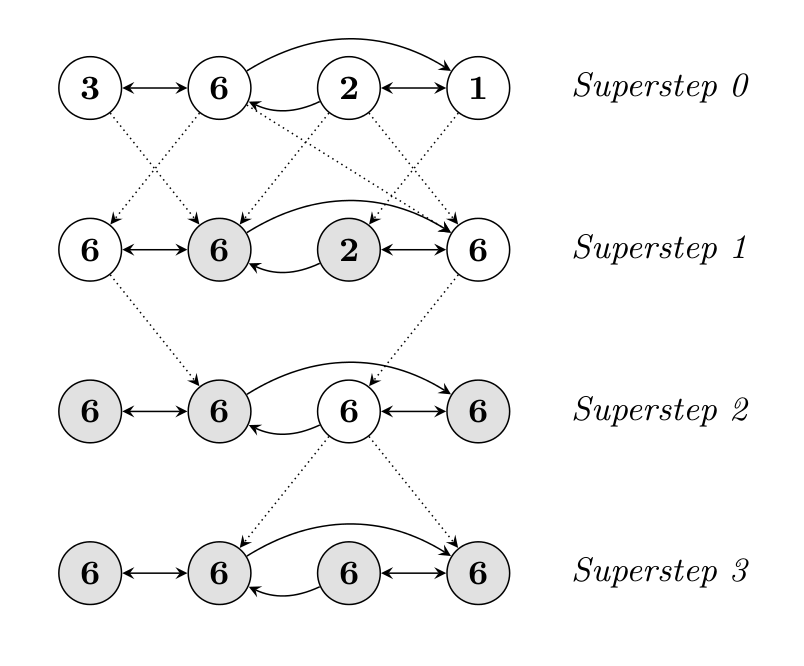
\includegraphics[width=0.6\textwidth]{PregelMaxVal.png}
\end{center}

For another example, let us see how single source shortest paths can be computed using Pregel. 
We assume that the value for each vertex is initially set to $\infty$.
In the first superstep the source vertex updates its value to $0$ and sends messages to its neighbors with a new distance. In the following supersteps,
other vertices update their distances and send messages to their neighbors with a new possible distance. Each vertex votes to halt in each superstep, so when no more messages with distance updates are sent, the algorithm terminates. This will always happen in a finite number of supersteps, as long as all edges have non-negative lengths. At the end of computation, each vertex has its minimum distance from \textit{SOURCE} associated with it, or $\infty$ if it is not reachable.

\begin{figure}[h!]
\parbox{0.8\textwidth}{
$\text{vertexProgram}(\textit{vertex, superstepNumber, incomingMessages}) \{$

~~~~$\textit{initialDistance} \leftarrow \textbf{if }(vertex.id = SOURCE)~0~\textbf{else}~\infty$

~~~~$\textit{minDistance} \leftarrow \min(\textit{incomingMessages} \cup \{\textit{initialDistance}\})$;

~~~~\textbf{if} $\textit{newValue} < \textit{vertex.value}$ \textbf{then}

~~~~~~~~$\textit{vertex.value} \leftarrow \textit{minDistance}$

~~~~~~~~\textbf{foreach} $\textit{edge} \in \textit{vertex.outgoingEdges}$ \textbf{do}

~~~~~~~~~~~~~~\text{sendMessage}$(\textit{edge.targetVertex, minDistance + edge.length})$;

~~~~\text{voteToHalt()};

$\}$
}

\caption{Pregel vertex program for shortest paths from \textit{SOURCE} to all other vertices}
\end{figure}


An important goal in large dataset computations is to achieve fault-tolerance, so the computation can be continued in case of a failure of some of the machines in the cluster. In Pregel, this is achieved by \emph{checkpointing}. Once in a few supersteps, the workers are required to save their state to the disk. When any of the workers fails, the computation is resumed from the last checkpoint.

In addition to the general model, Pregel also has some additional features enhancing usability and efficiency, such as \emph{aggregators} for efficiently gathering and broadcasting global values and \emph{combiners} which can reduce the network bandwidth used by merging messages send from vertices placed on a given node.

The original implementation by Google engineers is proprietary and was never released to the public. It is written entirely in C++ and tightly connected to the internal Google infrastructure, including the distributed file systems and execution environment.

\section{Giraph}

Giraph\cite{giraph} is an open-source implementation of the Pregel model.

Giraph is built on top of Hadoop \cite{hadoop}, the widely-adopted framework for large datasets processing. Hadoop is a platform for big datasets computing at scale, consisting of HDFS --- distributed file system, YARN --- framework for managing the cluster and scheduling tasks, Hadoop MapReduce --- an open implementation of the MapReduce model and libraries for using these elements in other projects.



\todo{
Giraph was
initially developed at Yahoo! and it was incubated at the Apache Foundation during summer
2011. In 2012 Giraph was promoted as Apache Top Level Project. Giraph is a (open source)
loose implementation of Google Pregel, and it is released under the Apache License. In 2013
the 1.0 version was released, as a proof of its stability and the number of features added
since its initial release. Giraph enlists contributors by Facebook, Twitter, LinkedIn, and it is
currently used in production at some of these companies and others. Giraph shares with
Pregel its computational model and its programming paradigm, but it extends the Pregel API
and architecture by introducing a Master compute function, out-of-core capabilities, etc., and
removing the single-point-of-failure (SPoF) represented by the master.
}
\todo{
Web and online social graphs have been rapidly growing in size and scale during the past decade. In 2008, Google estimated that the number of web pages reached over a trillion. Online social networking and email sites, including Yahoo!, Google, Microsoft, Facebook, LinkedIn, and Twitter, have hundreds of millions of users and are expected to grow much more in the future. Processing these graphs plays a big role in relevant and personalized information for users, such as results from a search engine or news in an online social networking site.
Graph processing platforms to run large-scale algorithms (such as page rank, shared connections, personalization-based popularity, etc.) have become quite popular. Some recent examples include Pregel and HaLoop. For general-purpose big data computation, the map-reduce computing model has been well adopted and the most deployed map-reduce infrastructure is Apache Hadoop. We have implemented a graph-processing framework that is launched as a typical Hadoop job to leverage existing Hadoop infrastructure, such as Amazon's EC2. Giraph builds upon the graph-oriented nature of Pregel but additionally adds fault-tolerance to the coordinator process with the use of ZooKeeper as its centralized coordination service.
Giraph follows the bulk-synchronous parallel model relative to graphs where vertices can send messages to other vertices during a given superstep. Checkpoints are initiated by the Giraph infrastructure at user-defined intervals and are used for automatic application restarts when any worker in the application fails. Any worker in the application can act as the application coordinator and one will automatically take over if the current application coordinator fails.}

różnce: master compute, out of core (na dysku)


\section{Spark}
Spark with GraphX

\section{Other extensions}
Giraph++



\chapter{SociaLite}\label{r:socialite}

\todo{zastanów się co w jakiej kolejności jest najważniejsze (i zrozumiałe dla czytelnika)}

SociaLite (\cite{socialite, distsoc}) is a graph query language based on Datalog. While Datalog allows to express some of graph algorithms
in an elegant and succinct way, many practical problems cannot be efficiently solved with Datalog programs. 

SociaLite allows a programmer to write intuitive queries using declarative semantics, which can often be executed as efficiently as highly optimized dedicated programs. The queries can then be executed in a distributed environment.

Most significant extension over Datalog in SociaLite is the ability to combine recursive rules with aggregation. Under some conditions, such rules can be evaluated incrementally and thus as efficiently as regular recursion in Datalog.

\cite{socialite} introduces \emph{Sequential SociaLite}, intended to be executed on one machine, consisting of two main extensions: \emph{recursive aggregate functions} and \emph{tail-nested tables}. Recursive aggregate functions are the most important feature in Socialite -- in \ref{s:recaggr} we present a complete definition and proofs of correctness of that extension, which are missing in \cite{socialite}. Tail-nested tables are a much more straightforward extension -- an optimization of data layout in memory. They are described in \ref{s:tnt}

\cite{distsoc} extends Sequential Socialite to \emph{Distributed SociaLite}, executable on a distributed architecture. It introduces a \emph{location operator}, which determines how the data and computations can be distributed. The programmer does not have to think about how to distribute the data between machines or manage the communication between them. He only specifies an abstract \emph{location} for each row in the data, and the data and computations are automatically sharded. Distributed SociaLite is covered in section \ref{s:distributed}

Additionally, thanks to the declarative semantics of Datalog and SociaLite, it is possible to provide an important optimization: the \emph{delta stepping} technique, which is an effective way of parallelizing the Dijkstra algorithm \cite{deltastep}. In SociaLite, this technique can be applied automatically to a certain class of recursive aggregate programs. \todo{zostaw sobie TODO i zastanówi się czy to dasz radę zrobić (potrzebny tu komentarz)
Być może będzie oddzielny rozdział o optymalizacji i te akapity wylądują tam (że oni robili to i to, a ty to i to, bo bardziej pasowało). Wtedy tu wystarczy wspomnieć że w socialite je mają.}

In distributed computations on large graphs, an approximate result is often enough. Usually we can observe the \emph{long tail} phenomenon in the computation, where a good approximate solution is achieved quickly, but it takes a long time to get to the optimal one. In SociaLite, by simply stopping the computation, we can obtain an approximate solution found so far. \cite{distsoc} also shows a method which can significantly reduce memory requirements by storing the intermediate results in an approximate way using Bloom filters. Those topics are covered in section \ref{s:approxdist} \todo{to np. nie będzie jasne dopóki nie wiemy więcej}

\section{Datalog with recursive aggregate functions}\label{s:recaggr}

In this section we introduce the recursive aggregate functions extension from SociaLite. Since the original SociaLite consists of several extensions to Datalog, we will call the language defined here \emph{Datalog with recursive aggregate functions}, abbreviated \datalogra.

\subsection{Motivation}
Most graph algorithms are essentially some kind of iteration or recursive computation. Simple recursion can be expressed easily in Datalog. However, in many problems the computation results are gradually refined in each iteration, until the final result is reached. Examples of such algorithms are the Dijkstra algorithm for single source shortest paths or PageRank. Usually, it is difficult or impossible to express such algorithms in Datalog efficiently, as it would require computing much more intermediate results than it is actually needed to obtain the solution. We will explain that on an example: a simple program that computes shortest paths from a source node.

A straightforward Datalog program for computing single source shortest paths (starting from node $1$) is presented below. Due to limitations of Datalog, this program computes all possible path lengths from node $1$ to other nodes in the first place, and after that for each node the minimal distance is chosen. Not only this approach results in bad performance, but causes the program to execute infinitely if a loop in the graph is reachable from the source node. \todo{czy to jest w Datalogu?
trzeba wyjaśnić że to już jest rozszerzenie a teraz tylko chodzi o sposób wyliczania i zapętlanie}

\dprog{}{
  & \textsc{Path} (t, d) &&  & \assign & && \textsc{Edge} (1, t, d). & \\
  & \textsc{Path} (t, d) &&  & \assign & && \textsc{Path} (s, d_1), \textsc{Edge} (s, t, d_2), d = d_1 + d_2. & \\
  & \textsc{MinPath} (t, \textsc{Min}(d)) &&  & \assign & && \textsc{Path} (t, d). &
}{Datalog query for computing shortest paths from node 1 to other nodes}{ex:ssspdatalog}

\datalogra allows aggregation to be combined with recursion under some conditions. This allows us to write straightforward programs for such problems, which finish execution in finite time and often are much more efficient than Datalog programs. An example \datalogra program that computes single source shortest paths is presented below. The relation $\textsc{Path}$ is declared so that for each \textit{target} the values in \textit{dist} column are aggregated using minimum operator.


\dprog{
  $\textsc{Edge}(\text{int } \textit{src}, \text{int } \textit{sink}, \text{int } \textit{len}) $ \\
  $\textsc{Path}(\text{int } \textit{target}, \text{int } \textit{dist} \text{ aggregate } \textsc{Min}) $
}{
  & \textsc{Path} (1, 0). &&  & & &&  & \\
  & \textsc{Path} (t, d) &&  & \assign & && \textsc{Path} (s, d_1), \textsc{Edge} (s, t, d_2), d = d_1 + d_2. &
}{SociaLite query for computing shortest paths from node 1 to other nodes}{ex:ssspsocialite}

While being very useful, recursive aggregation rules not always have an unambiguous solution. This is the case only under some conditions on the rules and the aggregation function itself.

Typically, Datalog programs semantics is defined using the fixed point of instance inclusion. This requires that the subsequent computation iterations only add tuples to the database instance, but never remove tuples from the instance. This is the reason for which program \ref{ex:ssspdatalog} is inefficient. When recursive aggregate functions are allowed, this is not the case: a tuple in the instance can be replaced with a different one because a new aggregated value appeared. Consequently, in order to define SociaLite programs semantics in terms of fixed point, we need to use a different order on database instances.

First, we will define a meet operation and show the order that it induces. Then we will show that if the aggregation function is a meet operation and corresponding rules are monotone with respect to this induced order, then the result of the program is unambiguously defined. We will also show how it can be computed efficiently.

\subsection{Meet operation and induced ordering}
\begin{defn}
A binary operation is a \emph{meet} operation if it is idempotent, commutative and associative.
\end{defn}
\todo{Maybe remind definitions of semi-lattice and partial order?}

\subsubsection{Order induced by a meet operation}

A meet operation $\sqcap$ defines a semi-lattice: it induces a partial order $\preceq_\sqcap$ over its domain, such that the result of the operation for any two elements is the least upper bound of those elements with respect to $\preceq_\sqcap$

\begin{exmp}
$\max(a, b)$ for $a, b \in \mathbb{N}$ is a meet operation; it is:
\begin{itemize}
\item idempotent -- $\max(a, a) = a$
\item commutative -- $\max(a, b) = \max(b, a)$
\item associative -- $\max(a, \max(b, c)) = \max(\max(a, b), c)$
\end{itemize}
It induces the partial order $\le$: for any two $a, b \in \mathbb{N}$, $\max(a, b)$ is their least upper bound with respect to $\le$.


On the contrary, $+$ is not a meet operation, since it is not idempotent: $1+1 \ne 1$.
\end{exmp}

\subsection{A program in \datalogra}
A \datalogra program is a Datalog program, with additional aggregation function defined for some of the relations:
For each relation $R$, there can be one column $\aggcol_R \in {1, \dots ar_R}$ chosen for which an aggregation function $\aggfun_R$ is provided. The rest of the columns are called the \emph{qualifying columns}. Intuitively, after each step of computation, we group the tuples in the relation by the qualifying columns and aggregate the column $\aggcol_R$ using $\aggfun_R$. Value $\aggcol_R = \bf{none}$ means that $R$ is a regular relation with no aggregation.

For simplicity, we assume that if a relation has an aggregated column, then it is always the last one: $\aggcol_R = ar_R$.

Syntactically, we require that each relation is declared at the top of the program as on the example below. In declaration of a relation, aggregated column can be specified by adding keyword \textit{aggregate} and name of the aggregate function next to the column declaration.

\begin{figure}[h!]
\narrow{
  $\textsc{P}(\text{int } \textit{a}, \text{int } \textit{b} \text{ aggregate } \textsc{F}) $\\
  $\textsc{R}(\text{int } \textit{src}, \text{int } \textit{sink}, \text{int } \textit{len}) $ 
  \begin{flalign*}
  & \textsc{P} (x_1, \dots, x_{ar_P}) &&  & \assign & && Q_{P,1}(x_1, \dots, x_{ar_P}) & \\
  &  &&  & \dots & && & \\
  & \textsc{P} (x_1, \dots, x_{ar_P}) &&  & \assign & && Q_{P,m}(x_1, \dots, x_{ar_P}) & \\
  & \textsc{R} (x_1, \dots, x_{ar_R}) &&  & \assign & && Q_{R,1}(x_1, \dots, x_{ar_R}) & \\
  &  &&  & \dots & && & \\
  & \textsc{R} (x_1, \dots, x_{ar_R}) &&  & \assign & && Q_{R,m}(x_1, \dots, x_{ar_R}) & \\
  \end{flalign*}
  \caption{Structure of a program in \datalogra.}
}
\end{figure}

\subsubsection{Aggregation operation $g_R$}
An important step in the evaluation of a \datalogra program is grouping the tuples in an instance of each relation and performing the aggregation within each group. We can put that into a formal definition as function $g_R$, which takes a relation instance which may contain multiple tuples with the same set of qualifying parameters and performs the aggregation.
\begin{defn}\label{d:aggregationoperationgr}
For a relation $R$ of arity $ar_R = k$, in let us define $g: \bf{dom}^k \to \bf{dom}^k$:
$$
g_R(I) = \begin{cases}
\{(x_1, \dots, x_{k-1}, \aggfun_R(\{y: (x_1, \dots, x_{k-1}, y) \in I\}): (x_1, \dots, x_{k-1}, x_k) \in I\} & \text{if } \aggcol_R \ne \bf{none} \\
I & \text{otherwise}
\end{cases}
$$
\end{defn}

If $R$ has an aggregated column, $g_R$ groups the tuples in relation instance $I$ by qualifying parameters and performs the aggregation using $\aggfun_R$. For non-aggregated relations, $g_R$ is an identity function.

\subsubsection{Order on relation instances}
In Datalog, we can prove that there is a unique least fixed point for any program. The fundamental fact needed for this proof is that during the evaluation of a Datalog program, if the state of a relation is $I_1$ at some point and $I_2$ at some other point, we know that $I_1 \subseteq I_2$. In \datalogra this property no longer holds: a tuple in $I_1$ can be replaced with different tuple with a lower value in the aggregated column. To be able to define semantics of programs in \datalogra using least fixed point, we need to use a custom order on relation instances.

\begin{defn}
Let $R$ be a relation. Let us define comparison $\sqsubseteq_R$ on relation instances as follows:
\begin{align}
I_1 \sqsubseteq_R I_2 \iff \forall_{(q_1, ..., q_{n-1}, v) \in g_R(I_1)} \exists_{(q_1, ..., q_{n-1}, v') \in g_R(I_2)} v \preceq_{\aggfun_R} v' & \text{ if } \aggcol_R \ne \bf{none} \\
I_1 \sqsubseteq_R I_2 \iff \forall_{(q_1, ..., q_n) \in g_R(I_1)} \exists_{(q_1, ..., q_n) \in g_R(I_2)} & otherwise
\end{align}
\end{defn}

\begin{note}
If $R$ does not have an aggregated column, $g_R(I) = I$ for any $I$, so $\sqsubseteq_R$ is simply the inclusion order $\subseteq$. 
\end{note}

\begin{lem}
For any $R$, $\sqsubseteq_R$ is a partial order.
\end{lem}

\emph{Proof:}

If $R$ does not have an aggregated column, $\sqsubseteq_R$ is the same as inclusion order $\subseteq$, which is a partial order.

If $R$ does have an aggregated column, then:

\begin{itemize}
\item $\sqsubseteq_R$ is reflexive: for each $R$, we have that  $\forall_{(q_1, ..., q_{n-1}, v) \in g(R)} \exists_{(q_1, ..., q_{n-1}, v) \in g(R)} v \preceq_{\aggfun_R} v $ because $\preceq_{\aggfun_R}$ is reflexive. Hence, $R \sqsubseteq_R R$.
\item $\sqsubseteq_R$ is antisimmetric \todo{No, it is not antisimmetric, so this is not a partial order --- how to deal with that?}
\item $\sqsubseteq_R$ is transitive: if $A \sqsubseteq_R B$ and $B \sqsubseteq_R  C$, then $\forall_{(q_1, ..., q_{n-1}, a) \in g(A)} \exists_{(q_1, ..., q_{n-1}, b) \in g(B)} a \preceq_{\aggfun_R} b $ and $\forall_{(q_1, ..., q_{n-1}, b) \in g(B)} \exists_{(q_1, ..., q_{n-1}, c) \in g(C)} b \preceq_{\aggfun_R} c$.

$\preceq_{\aggfun_R}$ is transitive, so $\forall_{(q_1, ..., q_{n-1}, a) \in g(A)} \exists_{(q_1, ..., q_{n-1}, c) \in g(C)} a \preceq_{\aggfun_R} c $, which means that $A \sqsubseteq_R C$.
\end{itemize}

\todo{Because of lack of antisimmetry it is only a preorder, not a partial order ---> how to deal with that?}

\todo{dodatkowy komentarz?}

\begin{exmp}
Let $R$ be a relation with arity $3$, with the last column aggregated using meet operation $\max$.
We recall that for $ \max $, $ \preceq_{\max} $ is the usual order $ \le $.
\begin{itemize}
\item $\{(1, 2, 3)\} \sqsubseteq_R \{(1, 2, 5)\}$, because $3 \le 5$
\item $\{(1, 2, 3)\} \sqsubseteq_R \{(1, 2, 5), (1, 7, 2)\}$ , because $3 \le 5$
\item $\{(1, 2, 3), (1, 2, 8)\} \sqsubseteq_R \{(1, 2, 5)\}$ , because $g_R(\{(1, 2, 3), (1, 2, 8)\}) = \{(1,2,3)\}$ and $3 \le 5$
\item $\{(1, 2, 3), (2, 8, 1)\}$ and  $\sqsubseteq_R \{(1, 2, 5), (1, 7, 2)\}$ are not comparable
\item $\emptyset \sqsubseteq_R \{(1, 2, 3)\}$
\end{itemize}
\end{exmp}

We can easily see that for any $R$ an empty relation instance $\emptyset$ is smaller under $\sqsubseteq_R$  than any other relation instance.


\subsection{Semantics and evaluation - one relation case}\label{ss:semeval1rel}
In this section we will show that the semantics of a \datalogra program can be unambiguously defined using least fixed point, as long as it satisfies some conditions. To simplify the reasoning, we will restrict our attention to programs with only one \emph{idb} relation. In the following section we extend the definitions and theorems presented here to the general case of many \emph{idb} relations.

Let $P$ be a \datalogra program, with only one \emph{idb} relation $R$ of arity $k$ in the form of:

\begin{figure}[h!]
\narrow{
%  $\textsc{R}(x_1, \dots, x_{k-1}, x_k [\text{ aggregate } \textsc{F}]) $\\
  \begin{flalign*}
  & \textsc{R} (x_1, \dots, x_k) &&  & \assign & && Q_1(x_1, \dots, x_k) & \\
  &  &&  & \dots & && & \\
  & \textsc{R} (x_1, \dots, x_k) &&  & \assign & && Q_m(x_1, \dots, x_k) & \\
  \end{flalign*}
}
\end{figure}

$Q_1, \dots, Q_m$ are rule bodies with free variables $x_1, \dots, x_k$. They may contain references to any of the \emph{edb} relations, which are constant during the evaluation or to the only \emph{idb} relation, $R$. We denote evaluation of rule body $Q$ in the context of an instance $I$ of the relation $Q$ as $E_I(Q)$.

Since we consider only one relation $R$, we can simplify the notation: let $\sqsubseteq$ denote $\sqsubseteq_R$ and let $g$ denote the aggregation operation $g_R$ for relation $R$, as defined in Definition \ref{d:aggregationoperationgr}.

Let us define $f: \bf{dom}^k \to \bf{dom}^k$ as the function that evaluates the rules $Q_1, ... Q_m$ based on the given instance of the relation $R$ and and returns its input extended with the set of generated tuples:
$$ f(I) = I \cup \bigcup_{i=1..m} E_I(Q_i) $$

Let $h = g \circ f$. 


\begin{thm}
If $f$ is monotone with respect to $\sqsubseteq$, i.e. $R_1 \subseteq R_2 \rightarrow f(R_1) \subseteq f(R_2)$, and there exists $n \ge 0 $, such that $h^n(\emptyset) = h^{n+1}(\emptyset)$, then $R^* = h^n(\emptyset)$ is the least fixed point of $h$, that is:
\begin{enumerate}
\item $R^* = h(R^*)$, i.e. $R^*$ is a fix-point
\item $R^* \sqsubseteq R$ for all $R$ such that $R = h(R)$, i.e. $R^*$ is smaller than any other fix-point
\end{enumerate}
\end{thm}

\emph{Proof:} 

$g$ is monotone with respect to $\sqsubseteq$. Since we assumed that $f$ is monotone with respect to $\sqsubseteq$, $h = g \circ f$ is also monotone with respect to $\sqsubseteq$. 

We know that $\emptyset$ is smaller under $\sqsubseteq$ than any other element.

Let us suppose that $I'$ is any fix-point of $h$.  We know that $\emptyset \sqsubseteq I'$. Applying $h$ to both sides of the inequality $n$ times, we have that $I^* = h^n(\emptyset) \sqsubseteq h^n(I') = I'$, thanks to the monotonicity of $h$ with respect to $\sqsubseteq$. Therefore, the inductive fixed point $I^*$ is the least fixed point of $h$.

In pseudocode, the evaluation algorithm is straightforward:

\begin{figure}[h!]
\narrow{
$I_0 \leftarrow \emptyset$

$i \leftarrow 0$

do

{\addtolength{\leftskip}{5mm}

$i \leftarrow i + 1$

$I_i \leftarrow h(I_{i-1})$

}

while $I_i \ne I_{i-1}$


\caption{Naive evaluation algorithm for \datalogra programs with one \textit{idb} relation.}
}
\end{figure}



\todo{open questions:
\begin{itemize}
\item How we compute recursive functions with non-meet aggregation operators? -- I can forbid that for now...
\end{itemize}
}


\begin{comment}

\subsection{Semi-naive evaluation -- one relation case}
\emph{Semi-naive evaluation} is the most basic optimization used in Datalog. In comes from the following observation: in a Datalog program, if some rule $Q$ produced a tuple $t$ based on database instance $I_i$ in the $i$-th iteration of the naive evaluation algorithm, then this rule with produce this tuple in each subsequent iteration, because $I_j \supseteq I_i$ for $j > i$. The goal of this optimization is to avoid such redundant computation. It is achieved by joining only subgoals in the body of each rule which have at least one new answer produced in the previous iteration.

In this section we give the algorithm for semi-naive evaluation in \datalogra and show that this optimization is valid.

\subsubsection{Algorithm}

\begin{figure}[h!]
\narrow{
$R_0 \leftarrow \emptyset, \Delta_0 \leftarrow \emptyset$

$i \leftarrow 0$

do

{\addtolength{\leftskip}{5mm}

$i \leftarrow i + 1$

$T_i \leftarrow \bigcup_{l=1..n} f(R_{i-1})$

$R_i \leftarrow g_k(T_i \cup R_{i-1})$

$\Delta_k^i \leftarrow R_k^i - R_k^{i-1}$

}

while not for all $k$ $\Delta_k^i = \emptyset$

\caption{Semi-Naive evaluation algorithm for \datalogra programs with one \textit{idb} relation.}
}
\end{figure}

\end{comment}


\subsection{Semantics and evaluation - multiple relations case}
In this section we extend \datalogra semantics from \ref{ss:semeval1rel} to a general case of possibly many \emph{idb} relations.

Let $P$ be a \datalogra program, with $w$ \emph{idb} relations $R_1, R_2, \dots, R_w$ of arities $k_1, k_2, \dots, k_w$ respectively.

\begin{figure}[h!]
\narrow{
%  $\textsc{R}(x_1, \dots, x_{k-1}, x_k [\text{ aggregate } \textsc{F}]) $\\
  \begin{flalign*}
  & \textsc{R$_1$} (x_1, \dots, x_{k_1}) &&  & \assign & && Q_{1,1}(x_1, \dots, x_{k_1}) & \\
  &  &&  & \dots & && & \\
  & \textsc{R$_1$} (x_1, \dots, x_{k_1}) &&  & \assign & && Q_{1,{m_1}}(x_1, \dots, x_{k_1}) & \\
  &  &&  & \dots & && & \\
  & \textsc{R$_w$} (x_1, \dots, x_{k_w}) &&  & \assign & && Q_{w, 1}(x_1, \dots, x_{k_w}) & \\
  &  &&  & \dots & && & \\
  & \textsc{R$_w$} (x_1, \dots, x_{k_w}) &&  & \assign & && Q_{w, {m_w}}(x_1, \dots, x_{k_w}) & \\
  \end{flalign*}
}
\end{figure}

For $i = 1, \dots, w$, $Q_{i,1}, \dots, Q_{i,m}$ are rule bodies with free variables $x_1, \dots, x_{k_w}$. They may contain references to the \emph{idb} relations $R_1, R_2, \dots R_w$ and the \emph{edb} relations, which are constant during the evaluation. We denote evaluation of rule body $Q$ in the context of an instance $I_1, \dots I_w$ of the relation $R_1, \dots, R_w$ as $E_(I_1, \dots, I_w)(Q)$.

For $i = 1, \dots, w$, $Q_{i,1}, \dots, Q_{i,m}$, let us define $f_i: P(\bf{dom}^{k_1}) \times \dots \times P(\bf{dom}^{k_w}) \to P(\bf{dom}^{k_i})$ as the function that evaluates the rules $Q_{i,1}, ... Q_{i, m_w}$ for relation $R_i$ based on the given instances of the relations $R_1, \dots, R_w$:
$$ f_i(I_1, \dots I_w) = I_i \cup \bigcup_{i=1..{m_w}} E_(I_1, \dots, I_w)(Q_i) $$

Let $h_i = g_{R_i} \circ f_i$. Let $h(I_1, \dots, I_w) = (h_1(I_1, \dots, I_w), \dots, h_w(I_1, \dots, I_w))$

Let $\sqsubseteq = \sqsubseteq_{R_1} \times \dots \sqsubseteq_{R_w}$.

\begin{thm}
If $h$ is monotone with respect to $\sqsubseteq$, i.e. $I \subseteq I' \rightarrow h(I) \subseteq f(I')$, and there exists $n \ge 0 $, such that $h^n(\emptyset) = h^{n+1}(\emptyset)$, then $I^* = h^n(\emptyset)$ is the least fixed point of $h$, that is:
\begin{enumerate}
\item $I^* = h(I^*)$, i.e. $I^*$ is a fix-point
\item $I^* \sqsubseteq I$ for all $I$ such that $I = h(I)$, i.e. $I^*$ is smaller than any other fix-point
\end{enumerate}
\todo{Extract the definition of fix-point -- it does not have to be here, but where to put it?}
\end{thm}

\emph{Proof:} 

We know that $\emptyset$ is smaller under $\sqsubseteq$ than any other element.

Let us suppose that $I'$ is any fix-point of $h$.  We know that $\emptyset \sqsubseteq I'$. Applying $h$ to both sides of the inequality $n$ times, we have that $I^* = h^n(\emptyset) \sqsubseteq h^n(I') = I'$, thanks to the monotonicity of $h$ with respect to $\sqsubseteq$. Therefore, the inductive fixed point $I^*$ is the least fixed point of $h$.

In pseudocode, the evaluation algorithm is straightforward:

\begin{figure}[h!]
\narrow{
$I_0 \leftarrow (\emptyset, \dots, \emptyset)$

$i \leftarrow 0$

do

{\addtolength{\leftskip}{5mm}

$i \leftarrow i + 1$

$I_i \leftarrow h(I_{i-1})$

}

while $I_i \ne I_{i-1}$

\caption{Naive evaluation algorithm for \datalogra programs with multiple \textit{idb} relations.}
}
\end{figure}


\todo{open questions:
\begin{itemize}
\item How we compute recursive functions with non-meet aggregation operators? -- I can forbid that for now...
\end{itemize}
}


\subsection{Semi-naive evaluation -- one relation case}
\emph{Semi-naive evaluation} is the most basic optimization used in Datalog evaluation. In comes from the following observation: in a Datalog program, if some rule $Q$ produced a tuple $t$ based on database instance $I_i$ in the $i$-th iteration of the naive evaluation algorithm, then this rule with produce this tuple in each subsequent iteration, because $I_j \supseteq I_i$ for $j > i$. The goal of this optimization is to avoid such redundant computation. It is achieved by joining only subgoals in the body of each rule which have at least one new answer produced in the previous iteration.

This optimization can be applied in \datalogra as well. To achieve this, we need to define function $f$ and the evaluation operation $E_I(Q)$ in a different way.




\subsection{\datalogra with negation}
\todo{Basically we do the same thing as in regular Datalog -- stratification}


\section{Tail-nested tables}\label{s:tnt}
Another important extension in SociaLite are \emph{tail nested tables}, which optimize the memory layout so that it can be accessed in a faster way. While being very useful in practice, this optimization is not crucial for running such programs on distributed architecture. \todo{I don't want to have this in the compiler, but maybe describe here?}

\section{Distributed SociaLite}\label{s:distributed}

\section{Delta stepping in Distributed SociaLite}\label{s:deltastep}

\section{Approximate evaluation in Distributed SociaLite}\label{s:approxdist}

\chapter{Translating SociaLite programs to Pregel}\label{r:s2p}

\chapter{Implementation}\label{r:implementation}

\chapter{Summary}\label{r:summary}


\begin{thebibliography}{99}
\addcontentsline{toc}{chapter}{Bibliografia}


\bibitem{socialite} Jiwon Seo, Stephen Guo, Monica S. Lam, \textit{SociaLite: Datalog extensions for efficient social network analysis}, ICDE 2013: 278-289

\bibitem{distsoc} Jiwon Seo, Jongsoo Park, Jaeho Shin, Monica S. Lam: \textit{Distributed SociaLite: A Datalog-Based Language for Large-Scale Graph Analysis}. PVLDB 6(14): 1906-1917 (2013)

\bibitem{fod} S. Abiteboul, R. Hull, and V. Vianu: \textit{Foundations of Databases}. Addison-Wesley (1995)

\bibitem{wfom} T.J. Ameloot, B. Ketsman, F. Neven, D. Zinn: \textit{Weaker Forms of Monotonicity for Declarative Networking: a more fine-grained answer to the CALM-conjecture}, PODS 2014

\bibitem{pagerank} S. Brin, L. Page. \textit{The anatomy of a large-scale hypertextual web search engine.} In WWW’98, 1998.

\bibitem{mapreduce} Jeffrey Dean , Sanjay Ghemawat: \textit{MapReduce: simplified data processing on large clusters}, Proceedings of the 6th conference on Symposium on Opearting Systems Design \& Implementation, 2004

\bibitem{pregel} Grzegorz Malewicz, Matthew H. Austern, Aart J.C. Bik, James C. Dehnert, Ilan Horn, Naty Leiser, Grzegorz Czajkowski: \textit{Pregel: a system for large-scale graph processing}, Proceedings of the 2010 ACM SIGMOD International Conference on Management of data, 2010

\bibitem{giraphpp} Y. Tian, A. Balmin, S. A. Corsten, S. Tatikonda, J. McPherson: \textit{From "Think Like a Vertex" to "Think Like a Graph"}, Proceedings of the VLDB Endowment, 2013

\bibitem{deltastep} U. Meyer, P. Sanders: \textit{Delta-stepping: A parallel
single source shortest path algorithm.} ESA, 1998.

\bibitem{ullman} Anand Rajaraman, Jeffrey D. Ullman: \textit{Mining of Massive Datasets}, Cambridge University Press, New York, NY, 2011

\bibitem{coddrelmodel} E. F. Codd: \textit{A relational model of data for large shared data banks}, Communications of the ACM, v.13 n.6, 1970

\bibitem{RBS87} R. Ramakrishnan, R. Bancilhon, A. Silberschatz:  \textit{Safety of recursive horn clauses with infinite relations}, Proc. ACM Symp. on Principles of Database Systems, 1987.
\bibitem{KRS88a} M. Kifer, R. Ramakrishnan, A. Silberschatz:  \textit{An axiomatic approach to deciding query safety in deductive databases}, Proc. ACM Symp. on Principles of Database Systems, 1988.
\bibitem{KRS88b} R. Krishnamurthy, R. Ramakrishnan, O. Shmueli:  \textit{A framework for testing safety and effective computability of extended Datalog}, Proc. ACM SIGMOD Symp. on the Management of Data, 1988.
\bibitem{SV89} Y. Sagiv, M. Y. Vardi:  \textit{Safety of datalog queries over infinite databases}.  Proc. ACM Symp. on Principles of Database Systems, 1989.

\bibitem{spark} Matei Zaharia, Mosharaf Chowdhury, Michael J. Franklin, Scott Shenker, Ion Stoica: \textit{Spark: Cluster Computing with Working Sets}, HotCloud 2010
\bibitem{pointanalysis} J. Whaley, M. S. Lam: \textit{Cloning-based context-sensitive pointer alias analyses using binary decision diagrams} In PLDI, 2004.
\bibitem{boomanalysis} P. Alvaro, T. Condie, N. Conway, K. Elmeleegy, J. M. Hellerstein, R. C. Sears: \textit{Boom analytics: Exploring data-centric, declarative programming for the cloud}, In EuroSys, 2010.
\bibitem{dataloganalysis} P. Alvaro, W. R. Marczak, N. Conway, J. M. Hellerstein, D. Maier, R. Sears. \textit{Dedalus: Datalog in time and space.} In Datalog, 2010

\bibitem{bsp} Leslie G. Valiant, \emph{A Bridging Model for Parallel Computation.} Comm. ACM 33(8), 1990, 103–111.

\bibitem{bgl} Jeremy G. Siek, Lie-Quan Lee, Andrew Lumsdaine: \textit{The Boost Graph Library: User Guide and Reference Manual.} Addison Wesley, 2002.
\bibitem{parallelbgl} Douglas Gregor, Andrew Lumsdaine: \textit{The Parallel BGL: A Generic Library for Distributed Graph Computations.} Proc. of Parallel Object-Oriented Scientific Computing (POOSC), July 2005.
\bibitem{GraphBase} Donald E. Knuth: \textit{Stanford GraphBase: A Platform for Combinatorial Computing.} ACM Press, 1994.

\bibitem{logicblox} http://www.logicblox.com/technology.html, Accessed: September 18th, 2014
\bibitem{datomic} http://www.datomic.com, Accessed: September 18th, 2014
\bibitem{giraph} http://giraph.apache.com, Accessed: September 18th, 2014
\bibitem{sparkwww} http://spark.apache.com, Accessed: September 18th, 2014
\bibitem{hadoop} http://hadoop.apache.com, Accessed: September 18th, 2014


\bibitem{magicsetsexist} Mario Alviano, Nicola Leone, Marco Manna, Giorgio Terracina, Pierfrancesco Veltri: \textit{Magic-Sets for Datalog with Existential Quantifiers.} Datalog 2012: 31-43
\bibitem{disjunctivedatalog} Mario Alviano, Wolfgang Faber, Nicola Leone, Marco Manna: \textit{Disjunctive datalog with existential quantifiers: Semantics, decidability, and complexity issues.} TPLP 12(4-5): 701-718 (2012)
\bibitem{datalogrelaunched} Francois Bry, Tim Furche, Clemens Ley, Bruno Marnette, Benedikt Linse, Sebastian Schaffert: \textit{Datalog relaunched: simulation unification and value invention}, Proceedings of the First international conference on Datalog Reloaded, March 16-19, 2010, Oxford, UK
\bibitem{magicsets} Francois Bancilhon, David Maier, Yehoshua Sagiv, Jeffrey D Ullman: \textit{Magic sets and other strange ways to implement logic programs}. In Proceedings of the fifth ACM SIGACT-SIGMOD symposium on Principles of database systems (PODS '86). ACM, New York, NY, USA.
\bibitem{subsumptivequeries} K. Tuncay Tekle, Yanhong A. Liu: \textit{More efficient datalog queries: subsumptive tabling beats magic sets.} In Proceedings of the 2011 ACM SIGMOD International Conference on Management of data (SIGMOD '11). ACM, New York, NY, USA.

\bibitem{giraphbook} Claudio Martella, Roman Shaposhnik, Dionysios Logothetis: \textit{Giraph in Action}, Early access edition, http://www.manning.com/martella/

\end{thebibliography}

\todo{http://giraph.apache.org/literature.html}


\end{document}

